\documentclass[tikz,border=12pt]{standalone}
% Match the sans-serif font stack used by the Minimal Mistakes site theme.
% TeX Gyre Heros is the TeX-compatible Helvetica implementation.
\usepackage[T1]{fontenc}
\usepackage{tgheros}
\renewcommand{\familydefault}{\sfdefault}

\usetikzlibrary{arrows.meta,positioning}
\definecolor{pink}{HTML}{F72585}\definecolor{blue}{HTML}{4DABF7}\definecolor{green}{HTML}{51CF66}\definecolor{violet}{HTML}{B197FC}\definecolor{ink}{HTML}{E9ECEF}\definecolor{panel}{HTML}{211C1D}
\begin{document}
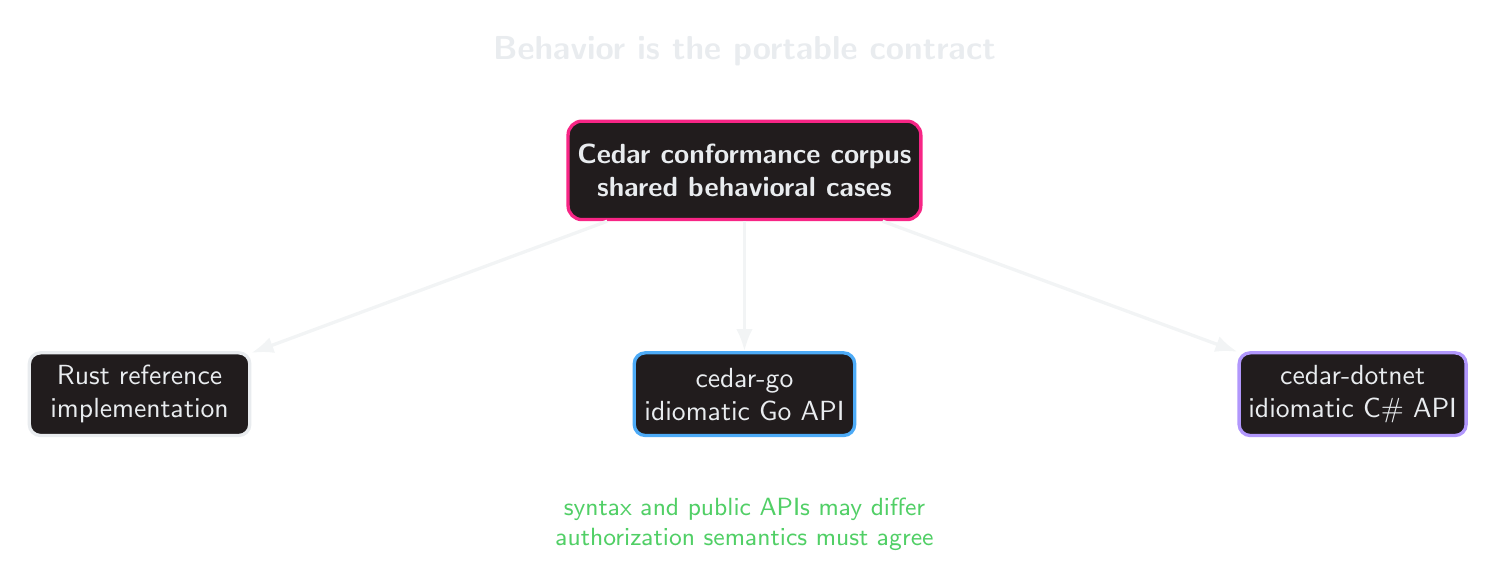
\begin{tikzpicture}[text=ink,impl/.style={rounded corners=4pt,fill=panel,very thick,minimum width=2.8cm,minimum height=1.05cm,align=center},arrow/.style={-{Latex[length=2.8mm]},very thick,ink!60}]
 \node[rounded corners=5pt,draw=pink,fill=panel,very thick,minimum width=4.3cm,minimum height=1.25cm,align=center,font=\bfseries] (corpus) {Cedar conformance corpus\\shared behavioral cases};
 \node[impl,draw=ink,below left=1.65cm and 4cm of corpus] (rust) {Rust reference\\implementation};
 \node[impl,draw=blue,below=1.65cm of corpus] (go) {cedar-go\\idiomatic Go API};
 \node[impl,draw=violet,below right=1.65cm and 4cm of corpus] (net) {cedar-dotnet\\idiomatic C\# API};
 \draw[arrow] (corpus)--(rust); \draw[arrow] (corpus)--(go); \draw[arrow] (corpus)--(net);
 \node[font=\small,align=center,text=green,below=.65cm of go] {syntax and public APIs may differ\\authorization semantics must agree};
 \node[font=\bfseries\large,text=ink,above=.55cm of corpus] {Behavior is the portable contract};
\end{tikzpicture}
\end{document}
